\documentclass[11pt,a4paper]{article}
\usepackage{ls}
\usepackage[english]{babel}
\setlist{noitemsep}

\title{Business Model Patterns and Sustainability}  

\author{Hans-Gert Gr\"abe}
\date{05 May 2022}

\begin{document}
\maketitle
\tableofcontents
\newpage

\section{Basics on Institutionalisation Processes}

\subsection{Dynamics of the Levels of Our Technology Definition}

Technology was defined in the lecture as interrelation of
\begin{itemize}
\item globally available \emph{procedural knowledge}, 
\item \emph{institutionalised procedures} ("state of the art") and
\item private \emph{procedural skills}.
\end{itemize}

The dynamics of these levels are closely linked:
\begin{enumerate}
\item Private procedural skills are based on institutionalised practices from
  which \emph{justified expectations} are derived.
\item The use of private procedural skills leads to \emph{experienced
  results}. Comparing them with justified expectations influences the
  institutionalisation of practically successful actions as proven practices.
\item This empiricism is \emph{condensed and generalised} as procedural
  knowledge extending it with appropriate conceptual systems, which in turn
  has an influence on the further development of "reasonable" practices and
  their forms of institutionalisation as \emph{contexts of justification}.
\end{enumerate}

\subsection{Transformation of Practically Proven into Proven Practices}

The transformation of what is practically proven into proven practices follows
a general line:
\begin{enumerate}
\item Procedures are standardised as processes and thus become comparable.
\item Tools are developed to support the operation of these processes.
\item Problems in the operation of these procedures are analysed, solutions
  are generalised, the practically proven is condensed into \emph{patterns}
  and further into standards, norms and the \emph{state of the art}.
\end{enumerate}
The generalisation of isolated practices into patterns also plays a role in
the TRIZ process model (Fig. 1): Darrell Mann's \emph{Select} phase draws on
these generalised experiences, which, however, for the TRIZ \emph{user} only
play a role as proven practices. Scientific elaboration means both empirically
to consolidate these proven practices and to integrate them into broader
contexts of justification and to develop corresponding conceptual worlds.

\subsection{Patterns and Contexts}

These forms of institutionalisation are embedded as initially domain-specific
patterns in a \emph{domain-specific} methodology, for example as industry
sector-specific standards and thus are \emph{contextualised}.  These patterns
can be further generalised to cross-domain standards such as the APQC PCF as a
Cross-Industry Process Classification Framework \cite{APQC}.  However, this is
also \emph{not universally valid}, but contextualised itself, as it still
refers to organisations of a specific-general design.

\begin{center}
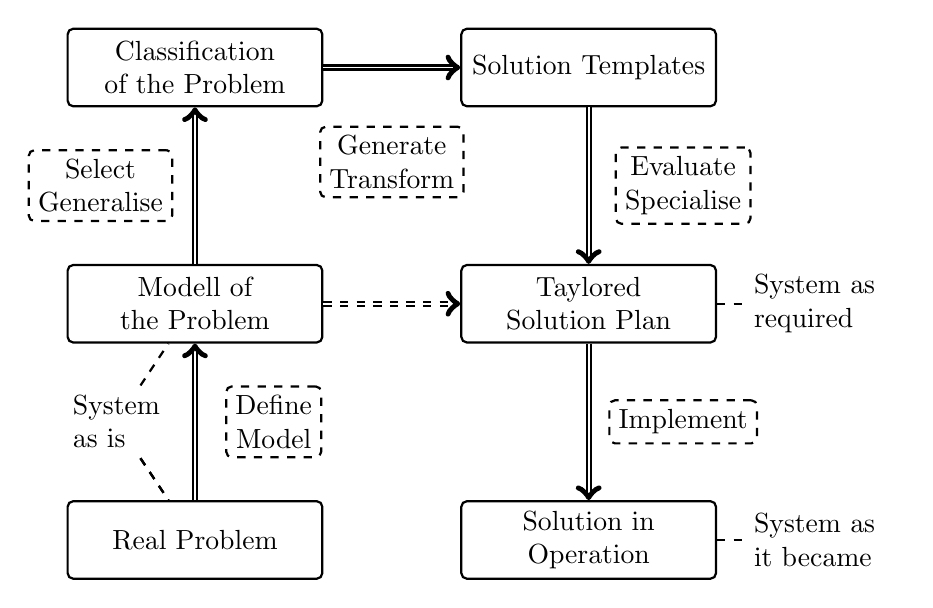
\begin{tikzpicture}[%scale=.95,transform shape,
    textbox/.style={draw, text width=3cm, minimum height=2.8em,
      align=center},
    ovalbox/.style={draw, dashed, align=center},
    %>={Triangle[length=0pt 6,width=0pt 5]},
    rounded corners=2pt,line width=.8pt]

  \node[text width=1.1cm] at (-1,1.5) (A0) {System\\ as is};
  \node[textbox] at (0,0) (A1) {Real Problem};
  \node[ovalbox] at (1,1.5) {Define\\ Model}; 
  \node[textbox] at (0,3) (A2) {Modell of the Problem};
  \node[ovalbox] at (-1.2,4.5) {Select\\ Generalise}; 
  \node[textbox] at (0,6) (A3) {Classification of the Problem};
  \node[ovalbox] at (2.5,4.8) {Generate\\ Transform}; 
  \node[textbox] at (5,6) (B3) {Solution Templates};
  \node[ovalbox] at (6.2,4.5) {Evaluate\\ Specialise}; 
  \node[textbox] at (5,3) (B2) {Taylored\\ Solution Plan};
  \node[ovalbox] at (6.2,1.5) {Implement}; 
  \node[textbox] at (5,0) (B1) {Solution in Operation};
  \node[text width=1.8cm] at (8,3) (C2) {System as\\ required};
  \node[text width=1.8cm] at (8,0) (C1) {System as\\ it became};

  \draw[-,dashed] (A0) -- (A1);
  \draw[-,dashed] (A0) -- (A2);
  \draw[-,dashed] (B1) -- (C1);
  \draw[-,dashed] (B2) -- (C2);
  \draw[-,dashed] (A0) -- (A1);
  \draw[-,dashed] (A0) -- (A1);

  \draw[double,->] (A1) -- (A2) ;
  \draw[double,->] (A2) -- (A3) ;
  \draw[double,->] (A3) -- (B3) ;
  \draw[double,->,dashed] (A2) -- (B2) ;
  \draw[double,->] (B3) -- (B2) ;
  \draw[double,->] (B2) -- (B1) ;
\end{tikzpicture}\\[1em]
Fig. 1: The TRIZ Process Model
\end{center}

\subsection{TRIZ and Patterns}

TRIZ is similarly structured. It comes with a toolbox of problem-solving
patterns (Select)
\begin{itemize}
\item 40 principles
\item 76 standards for SF models
\item Evolutionary patterns of technical systems
\item Evolutionary lines of technical systems
\end{itemize}
but assumes a specific type of modelling (Define) with
\begin{itemize}
\item systemic delimitation
\item ideality
\item focussing of an operative zone
\item action and evaluation parameters in functional modelling
\item Problems as contradictory behaviour of evaluation parameters when action
  parameters are changed.
\end{itemize}
Only on the basis of this (Define) is (Select) possible. It is also not only a
matter of \emph{selecting} the patterns suitable for the solution, but also of
\emph{selecting proven methodological procedures} that are based on the
respective patterns.
\newpage

\section{Development of Business Process Modelling}

When we talk about Business TRIZ today, we are talking about a similar
development of institutionalisation of structuring procedures in the area of
business processes.  In the context of P-TRIZ (Seminar on 9 May 2022), we had
identified three stages of that development:
\begin{enumerate}
\item With the transition to more advanced forms of industrial production at
  the beginning of the 20th century, individual work processes were
  deconstructed, charged with forms of description and assembled into new
  "living" systems -- the \emph{assembly line system} of modern industrial
  production. The control of the complex interrelationships in such an
  organisation remains as an "art of management" beyond the realm covered by
  these structural standardisation.

  At the centre of institutionalisation are complex engineering disciplines
  such as process engineering or automation technology, which are concerned
  not only with the processes themselves, but also the tools (understood in a
  comprehensive sense) that have been and are being created in the context of
  this institutionalisation.

  With its procedures and patterns, classical TRIZ aims at problem solving in
  this area. It can be applied only insofar as the concrete application domain
  is conceptually penetrated to such an extent that the specific type of
  modelling required in the TRIZ analysis phase can be carried out.  In this
  sense TRIZ is a "scientific method".

  "Management" remains an art, as in "Mintzberg on Management"
  \cite{Mintzberg}, for example, whereby an artist must certainly master the
  \emph{technical procedures} of his subject, but the practical combination of
  such techniques remains at the level of private procedural skills.
\item Since the 1960s, the structuring of procedures in the operational
  management of individual companies has gained in importance as
  \emph{business process modelling}.

  These institutionalisation processes are not possible without the preceding
  institutionalisations of the technical core processes and build on them.

  Howard Smith \cite{Smith2006} stated in 2006 that these institutionalisation
  processes are well advanced with the development and widespread use of
  computer-based business process management systems and the establishment of
  uniform conceptual systems such as the APQC PCF \cite{APQC}. This would
  allow us to move on to the next level, to \emph{P-TRIZ}.
  \begin{quote}
    P-TRIZ is the application of modern TRIZ towards business process
    improvement, innovation, and transformation. Coupled to BPM methods, it
    provides the engineering discipline that amplifies the creativity of those
    who seek to re-design processes. \cite{Smith2006}
  \end{quote}
\item In the management literature, this level of institutionalisation of
  structuring in inter-company cooperation has since been roughly associated
  with the term \emph{business model}. It is based on the forms of
  institutionalisation of intra-company operative business, but did not
  develop as quickly as Howard Smith expected at the time.
\end{enumerate}

\section{Business Process Models and Business Models}

\subsection{Business Process Models}

This confusion is also reflected in the literature consulted for the seminar.
In \cite{Fellmann2018}, "business process model patterns" are examined,
defined as
\begin{quote}
  the description of a proven solution to a recurring problem that is related
  to the creation or modification of business process models in a specific
  context. This description is typically organised in a structured document
  supporting the reader in understanding under which circumstances the
  proposed solution will be useful (ibid, p. 974),
\end{quote}
The authors clearly emphasise that 
\begin{quote}
  in economics the term \emph{business model patterns} is used for a pattern
  describing the economic principles of an organisation [\ldots] Although
  business model patterns can be depicted visually, they were not considered
  in our survey due to their specificity on the economics perspective.
\end{quote}
The aim of the work is described as to "discuss patterns related to various
aspects of process modeling" (ibib, p. 981). 15 years after \cite{Smith2006},
it is still about the third phase of the institutionalisation of patterns as a
central component of a problem-solving system in the field of Business Process
Landscapes of operational management.

\emph{Patterns} are understood in the sense of Christopher Alexander's
architecture patterns \cite{Alexander} or the Software design patterns of the
"Gang of Four" \cite{Gamma}.  In \cite[p. 3]{LF2018} this is defined as
follows
\begin{quote}
  A pattern is a combination of a problem and a corresponding solution that is
  described in a systematic and generic way, so that it can be used over and
  over again in different situations.
\end{quote}

This is not exactly the same as principles, evolutionary lines or trends in
TRIZ, as in these approaches there is no direct link between problem and
solution, but the "TRIZ model of the system as it is" is used as starting
point for selecting a systemic transformation pattern first to design the
solution in general and then to concretise it with available resources (phase
"Select" by Darrell Mann \cite{Mann} -- see the descriptions of the different
\emph{Problem Solving Tools} there).  They are nevertheless also subsumed as
"patterns" below. 

Business TRIZ has a nevertheless similar focus as business process models in
many practical applications in which it has to resolve contradictory
objectives in the operational organisation of the company. However, Business
TRIZ does not look for new patterns, but tries to transfer the patterns known
from the technical field to this field and adapt them on the basis of
experience gained. Such a transfer may seem suspicious at first glance.
However, it can be observed that essential instruments of classical TRIZ, such
as, e.g., the Patterns of Evolution of Technical Systems, are based on
observations on market processes and developments as explained in more detail
in \cite{Graebe2020} and thus have a certain relevance not only for the level
of Business Process Management Systems but also for the level of Business
Models.

\subsection{Business Models}

The level of business models has been studied more intensively since around
2010. In a first overview \cite{Zott2011} the authors observed "that scholars
do not agree on what a business model is, and that the literature is
developing largely in silos, according to the phenomena of interest to the
respective researchers" and present a list of eight different definitions of
the notion of a business model.  Nevertheless they identified emerging common
themes among scholars of that area:
\begin{enumerate}
\item The notion of business model is emerging as a new unit of analysis.
\item Business models emphasise a system-level, holistic approach towards
  explaining how firms “do business”.
\item Firm \emph{activities} play an important role in the various
  conceptualisations of business models that have been proposed.
\item Business models seek to explain how value is created, not just how it is
  captured. 
\end{enumerate}

This strong orientation towards value creation plays a central role in
\cite{Zott2011}, \cite{Remane2019}, but also in the much-cited reference
\cite{Gassmann2014}. Despite such a relatively homogeneous focus, however, no
generally accepted "Pattern Database" has yet emerged.  One problem is, of
course, the focus itself, since with \emph{value proposition} it is oriented
towards a functional property of the components and not towards a functional
property of the network, whose \emph{main useful function} should be an
emergent function of the network as a whole according to the theoretical
approach of TRIZ.

\section{Business Models and Sustainability}

In this sense, the concept of sustainability is a touchstone to what extent
Business Model Pattern taxonomies can address topics beyond such a narrow
focus.

Today's inclusion of sustainability issues in business models is largely the
result of a longer-term politicisation of this issue.

\subsection{Sustainability Emerging as Business Goal}

The importance of sustainable and ecological aspects in management has been a
topic of public awareness at least since the reports on the \emph{Limits to
  Growth} by the Club of Rome. While in the early years the debate focused on
the finite nature of available natural resources and thus on longer-term
development aspects of availability of a \emph{material basis} (such as "peak
oil"), in the last 20 years it has become increasingly visible that global
\emph{processes} (such as "climate change" or "extinction of species") will
leave familiar paths much earlier if the established industrial mode of
production which is the basis of our prosperity will be continued and further
expanded.

In contrast to other globalisation processes such as, e.g., the implementation
of Intellectual Property Rights, these processes do not originate and were
driven by individual interest groups, but have the \emph{cooperative action}
of an inherently global "thinking" of a networked, interdisciplinary science
as their basis. The problematisation was initiated and formed by international
bodies and today plays an increasingly important role in the framework of
international political affairs. The formula "think globally, act locally"
nevertheless expresses that those global challenges can only be met through
changed local action. Corresponding awareness-raising processes at the
socio-cultural and political level have meanwhile reached such a degree that
at least a financially potent middle class bases its economic decisions also
on ecological and social issues.

With the 17 Sustainable Development Goals (SDG) adopted in 2015 by the UN, the
politicisation of this issue has reached a new dimension, as these goals
anchor long-term objectives of necessary changes with today's cooperate
actions.

\begin{center}
  \begin{minipage}{.55\textwidth}\centering
    \includegraphics[width=\textwidth]{SDG.png}\\
    Sustainable Development Goals
  \end{minipage}\hfill
  \begin{minipage}{.4\textwidth}\centering
    \includegraphics[width=\textwidth]{Triple-Bottom-Line.png}\\[1em]
    Triple Bottom Line
  \end{minipage}

\end{center}

\subsection{Sustainability and Business Models}

In the business environment and more general socio-economic debates, this
politicisation is anchored with the slogan of the \emph{Triple Bottom Line:
  Planet -- People -- Profit} \cite{Elkington1997}. It obviously reveals
massive contradictory dimensions in the inclusion of ecological (planet) and
social (people) goals in economic processes.

Even if such a narrative is being further refined today with the PESTLE
approach (addressing the political, economical, social, technological, legal
and environmental dimensions), in view of the value orientation of Business
Model Pattern taxonomies so far, a consistent orientation towards all three
"P" can hardly be expected.

This main focus on value propositions is emphasised in \cite{LF2018} in the
introduction to the survey citing \cite{Schaltegger2016}:
\begin{quote}
  A business model for sustainability “helps describing, analyzing, managing,
  and communicating
  \begin{itemize}
  \item[(i)] a company’s sustainable value proposition to its customers, and
    all other stakeholders,
  \item[(ii)] how it creates and delivers this value,
  \item[(iii)] and how it captures economic value while maintaining or
    regenerating natural, social, and economic capital beyond its
    organizational boundaries”.
  \end{itemize}
\end{quote}
The authors identify 45 patterns extracted from the literature on Sustainable
Business Models and group them into 11 pattern groups 
\begin{itemize}
\item[G1] Pricing \& Revenue Patterns (4 patterns)
\item[G2] Financing Patterns (3 patterns)
\item[G3] Ecodesign Patterns  (4 patterns)
\item[G4] Closing-the-Loop Patterns (9 patterns)
\item[G5] Supply Chain Patterns (6 patterns)
\item[G6] Giving Patterns (2 patterns)
\item[G7] Access Provision Patterns (6 patterns)
\item[G8] Social Mission Patterns (5 patterns)
\item[G9] Service \& Performance Patterns (4 patterns)
\item[G10] Cooperative Patterns (1 pattern)
\item[G11] Community Platform Patterns (1 pattern)
\end{itemize}
As example the patterns in the group \emph{Pricing \& Revenue Patterns} are
listed: 
\begin{itemize}
\item Differential Pricing
\item Freemium
\item Innovative Product Financing
\item Subscription Model
\end{itemize}
For each of the patterns context, problem, solution are describes and an
example is given, e.g. for \emph{Differential Pricing}
\begin{itemize}
\item \emph{Context:} Base of the Pyramid and low-income groups in both
  developed and developing countries are often excluded from consumption due
  to price barriers.
\item \emph{Problem:} Customers might need the same product but have different
  payment thresholds. Hence, some customers are either unwilling or unable to
  pay as much as others for the same product.
\item \emph{Solution:} Charging groups with higher payment thresholds higher
  prices to subsidize those groups who cannot afford to pay as much.
\item \emph{Example:} [Novo Nordisk] sells insulin in developing countries at
  prices that are up to 20\% below the mean prices charged in developed
  countries.
\end{itemize}

The example shows very well the structured approach (the patterns as RDF are
meanwhile also part of the WUMM database), but also the extensive orientation
towards new and flexible forms of value proposition, which are driven more by
new possibilities emerging within digital change than by questions of
sustainability.  This is also emphasised in \cite[p. 3]{Russo2020}:
\begin{quote}
  General purpose idea generation tools do not usually show any specific
  preference to sustainable aspects, since their overall purpose is product
  success and the identification of unexplored market opportunities.
  Therefore, the attention to sustainability is random, not taken for granted
  and presumably dependent on designers’ sensibilities towards environmental
  and human problems.
\end{quote}


\subsection{Lifecycle Orientation and Eco Design Principles}

The approach in the works \cite{Russo2020} and \cite{Maccioni2019}, which
consider \emph{Eco Design Principles} (EDP), is clearly different. Here, the
focus is not on Business Models but on the Product Lifecycle and thus on
\emph{material processes} in their full complexity. Even if "market success as
key for any eco-design product" \cite[p. 1]{Maccioni2019} is emphasised, the
EDP are primarily directed at the early phases of product design.

The general orientation of EDP is described in \cite[p. 3]{Russo2020} as
follows:
\begin{quote}
  During design phase, each designer is supposed to follow a list of
  guidelines and accordingly modify the existing product to make it more
  environmentally friendly. The crucial point is to exploit problem solving
  strategies as a framework for eco-guidelines that guide the user to make
  product development, taking into account first of all sustainability
  objectives.

  It is important to understand that problem-solving tools are not easy to
  learn, so a strong simplification is needed to guide non-experts. Unlike a
  structured problem-solving method that involves a preliminary phase of
  understanding and modeling the problem, an eco-guideline acts exclusively as
  an inventive trigger. Therefore, it must be both simple to understand and
  effective.
\end{quote}

The aim of the EDP presented in \cite{Russo2020} is "the customization of a
set of tools that are typical of the TRIZ methodology. Almost all suggestions
are based on TRIZ tools [\ldots] However, TRIZ is not a method born to do
Ecodesign and, therefore, there has been a long work of selection and
adaptation of individual instruments. Only those instruments leading to
solutions with less waste of resources have been chosen."

16 generic strategies 
\begin{enumerate}
\item Switch to super system
\item Trimming
\item Dematerialization/ideality
\item Merging
\item Redesign the internal structure
\item Change the state of aggregation
\item Local quality
\item Substitute
\item Segmentation of the parts/components
\item Design for Assembly
\item Dynamics
\item The Other Way Around
\item Taking out
\item Increase control
\item Recycle/Reuse
\item Optimize
\end{enumerate}
are derived, to which the identified 59 Eco Guidelines are assigned. Each of
these generic strategies is embedded in the TRIZ methodology and their solving
power is outlined without, however, assigning them to a problem.  The authors
emphasise that they "have worked on the mechanisms of activation of creativity
that are typical of the TRIZ methodology, trying to translate it into
guidelines bypassing every step of problem definition." This is clearly
different to the "pattern approach" as developed, e.g., in \cite{LF2018}.

Instead, the description of each principle is limited to a detailed
\emph{Generic Suggestion}, more structured \emph{specific suggestions} and
examples.

Similar to \cite{Gassmann2014}, the individual EDPs are also assigned values
from a morphological table with the attributes \emph{when, action, what,
  how}.
\begin{itemize}
\item \emph{When:} Premanufacturing, Manufacturing, Use, End of Life
\item \emph{Action:} Eliminate, Reduce Mass, Reduce Volume, Reduce Quantity,
  Reduce Distance, Improve Durability, Select Other.
\item \emph{What:} Raw materials, External logistics, Internal logistics,
  Packaging, Machineries, Auxiliary materials, Components, Emissions, Energy.
\item \emph{How:} Generic suggestion, Resources list, Example.
\end{itemize}
The general pattern of a guideline can be formulated as 
\begin{quote}
  “(WHEN) you want to intervene, (ACT) on components (WHAT), by doing
  something (HOW) and using one resource (from the Resource list) to find
  alternatives and assess environmental impacts”.  
\end{quote}
In \cite[Fig. 2]{Russo2020} the following sample of a guideline is given: 
\begin{quote}
  During supply task (WHEN -- Premanufacturing),\\ reduce the mass (ACTION --
  Reduce mass)\\ of the raw material (WHAT -- Raw material)\\ by recycling
  waste material in your facility to make it new raw material for the product
  (HOW -- Generic Suggestion). \\
  See list of structural resources (HOW -- Resources list)\\
  In order to reduce the mass of the casting metal, the casting channels can
  be re-used for successive melting (HOW -- Example) 
\end{quote}



\begin{thebibliography}{xxx}
\bibitem{Alexander} Christopher Alexander, Sara Ishikawa, Murray Silverstein
  (1977). A Pattern Language: Towns, Buildings, Construction, Oxford
  University Press.

\bibitem{APQC} APCQ (2018). Cross Industry Process Classification Framework
  v.7.2.1
  
\bibitem{Elkington1997} John Elkington (1997). Cannibals with Forks: Triple
  Bottom Line of 21st Century Business

\bibitem{Fellmann2018} Michael Fellmann, Agnes Koschmider, Ralf Laue, Andreas
  Schoknecht, Arthur Vetter (2018).  Business Process Model Patterns:
  State-of-the art, Research Classification and Taxonomy.  Business Process
  Management Journal. \\ \url{https://doi.org/10.1108/BPMJ-01-2018-0021}
  
\bibitem{Gamma} Erich Gamma, Richard Helm, John Vlissides, Ralph Johnson
  (1994).Design Patterns: Elements of Reusable Object-Oriented Software.
  Addison Wesley.

\bibitem{Gassmann2014} Oliver Gassmann, Karolin Frankenberger, Michaela Csik
  (2020). The Business Model Navigator: 55 Models that will Revolutionise your
  Business. Harlow, UK: Pearson.

\bibitem{Graebe2020} Hans-Gert Gräbe (2020). Die Menschen und ihre Technischen
  Systeme (Human and their technical systems).  LIFIS ONLINE, 19.05.2020.
  \url{http://dx.doi.org/10.14625/graebe_20200519}

\bibitem{LF2018} Florian Lüdeke-Freund, Sarah Carroux, Alexandre Joyce,
  Lorenzo Massa, Henning Breuer (2018). The sustainable business model pattern
  taxonomy — 45 patterns to support sustainability-oriented business model
  innovation.  Sustainable Production and Consumption, Volume 15,
  pp. 145-162. \\ \url{https://doi.org/10.1016/j.spc.2018.06.004}
  
\bibitem{Maccioni2019} Lorenzo Maccioni, Yuri Borgianni, Daniela C. A. Pigosso
  (2019).  Can the choice of eco-design principles affect products’ success?
  Design Science, vol. 5, e25. \\ \url{https://doi.org/10.1017/dsj.2019.24}

\bibitem{Mann} Darrell Mann (2007). Hands-On Systematic Innovation for
  Business and Management.  IFR Press.

\bibitem{Mintzberg} Henry Mintzberg (1989). Mintzberg on Management.

\bibitem{Remane2019} Gerrit Remane, Andre Hanelt, Jan F. Tesch, Lutz M. Kolbe
  (2017).  The Business Model Pattern Database — A Tool for Systematic
  Business Model Innovation.  International Journal of Innovation Management
  Vol. 21 (1).\\ \url{https://doi.org/10.1142/S1363919617500049}
  
\bibitem{Russo2020} Davide Russo, Christian Spreafico (2020).  TRIZ-Based
  Guidelines for Eco-Improvement. Sustainability 2020, 12, 3412.
  \url{https://doi.org/10.3390/su12083412}

\bibitem{Schaltegger2016} Stefan Schaltegger, Florian Lüdeke-Freund, Erik
  G. Hansen (2016). Business Models for Sustainability: A Co-Evolutionary
  Analysis of Sustainable Entrepreneurship, Innovation, and Transformation.
  Organization \& Environment, 29(3), 264-289.

\bibitem{Smith2006} Howard Smith (2006). P-TRIZ in the History of Business
  Process. Part 3 in a series on P-TRIZ.  Computer Sciences Corporation.

\bibitem{Zott2011} Christoph Zott, Raphael Amit, Lorenzo Massa (2011). The
  business model: Recent developments and future research. Journal of
  management, 37 (4), 1019–1042.
  
\end{thebibliography}

\end{document}

